\section{The chosen neural network architectures}

\subsection*{The regular Autoencoder}

\begin{figure}[h!]
    \centering
    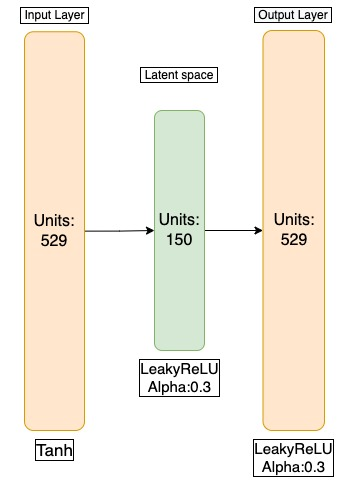
\includegraphics[scale=0.4]{Figures/nnarchitect/ae_small.jpeg}
    \caption[AE | Small network architecture]{Small autoencoder architecture.}
    \label{fig:ae_small}
\end{figure}

Figure \ref{fig:ae_small} shows the small autoencoder. It consists of an input and output layer of 529 nodes, with 
one latent space layer of 150 nodes. The activation functions for the input is Tanh while the latent space and the 
output layer use LeakyReLU with $\alpha=0.3$.


\begin{figure}[h!]
    \centering
    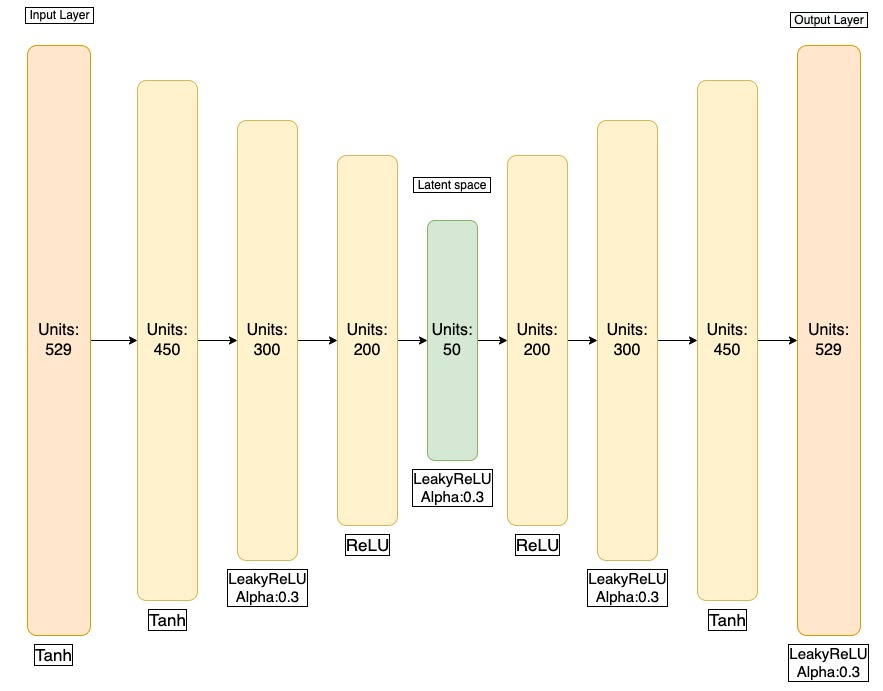
\includegraphics[width=0.8\textwidth]{Figures/nnarchitect/ae_big.jpeg}
    \caption[AE | Large network architecture]{Large autoencoder architecture.}
    \label{fig:ae_big}
\end{figure}

Figure \ref{fig:ae_big} shows the large regular autoencoder. It consists of an input and output layer of 529 nodes, with three 
hidden layers of 450, 300 and 200 nodes, respectively, in the encoder and three hidden layers of 200, 300 and 450 in the decoder, respectively. 
The activation functions for the input and ouput layers are the Tanh and LeakyReLU with $\alpha=0.3$. The encoder layers 
have the activation functions Tanh, LeakyReLU with $\alpha=0.3$ and ReLU. The decoder layers have the activation functions ReLU, 
LeakyReLU with $\alpha=0.3$ and Tanh. The latent space has 150 nodes,
with the LeakyReLU activation function with $\alpha=0.3$. The activation functions as well as the number of nodes per layer were chosen 
based on earlier work done 
on the ATLAS open data\cite{fys5555}, as well as some light hyperparameter testing using Keras-Tuner\cite{omalley2019kerastuner}.
\subsection*{The variational Autoencoder}
Figure \ref{fig:vae_small} and \ref{fig:vae_big} summarize the two models used for the variational autoencoder. 

\begin{figure}[h!]
    \centering
    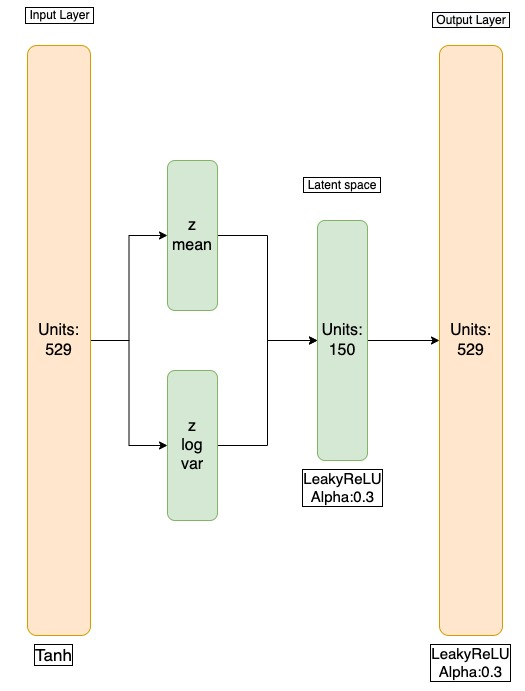
\includegraphics[scale=0.4]{Figures/nnarchitect/vae_small.jpeg}
    \caption[VAE | Small network architecture]{Small variational autoencoder architecture.}
    \label{fig:vae_small}
\end{figure}

In figure \ref{fig:vae_small} we have the small variational autoencoder. It consists of an input and output layer of 529 nodes, with 
one latent space layer of 150 nodes sampling from a mean and variance layer of same size. The activation functions for the input, latent space and  
output are the Tanh, LeakyReLU with $\alpha=0.3$ and Sigmoid, respectively. 

\begin{figure}[h!]
    \centering
    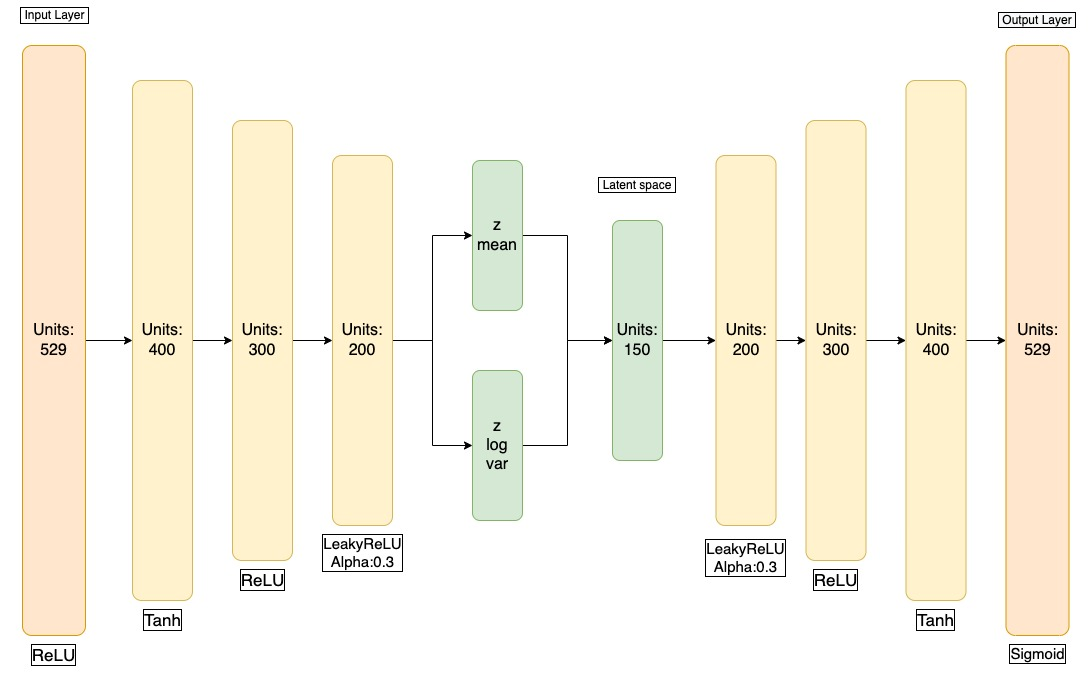
\includegraphics[width=0.8\textwidth]{Figures/nnarchitect/vae_big.jpeg}
    \caption{Large variational autoencoder architecture.}
    \label[VAE | Large network architecture]{fig:vae_big}
\end{figure}


The large variational autoencoder in figure \ref{fig:vae_big} consists of an input and output layer of 529 nodes, with three 
hidden layers of 400, 300 and 200 nodes respectively in the encoder and three hidden layers of 200, 300 and 400 in the decoder. 
The activation functions for the input and ouput layers are the ReLU and Sigmoid, respectively. The hidden 
layers in the encoder have the activation functions Tanh, ReLU, LeakyReLU with $\alpha=0.3$, respectively. The hidden layers
in the decoder have the activation functions LeakyReLU with $\alpha=0.3$, ReLU and Tanh, respectively. The activation functions 
as well as the number of nodes per layer were chosen based on earlier work done 
on the ATLAS open data\cite{fys5555}, as well as some light hyperparameter testing using Keras-Tuner\cite{omalley2019kerastuner}.